\chapter{Numerical Experiments}
\section{Constant Velocity}
\begin{figure}[H]
	\centering
	\begin{subfigure}{0.5\textwidth}
		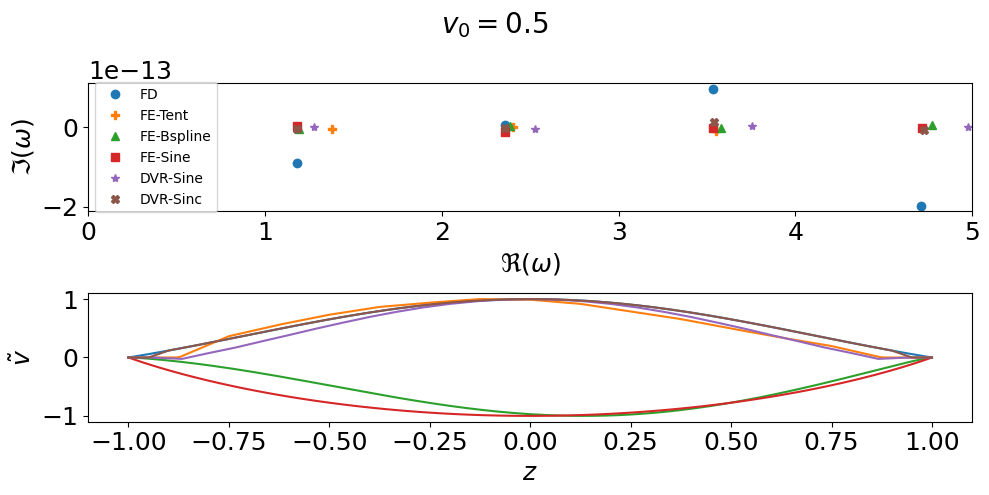
\includegraphics[width=\linewidth]{img/constant_v/constant-v-Mm=0.5}
		\caption{}
	\end{subfigure}%
	\begin{subfigure}{0.5\textwidth}
		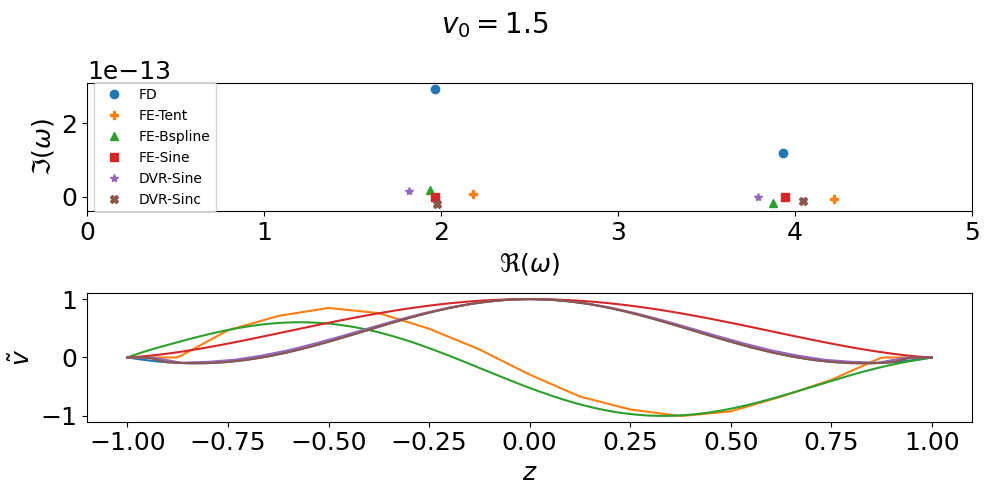
\includegraphics[width=\linewidth]{img/constant_v/constant-v-Mm=1.5}
		\caption{}
	\end{subfigure}
	\caption{In subsonic case, all methods produces stable modes. In supersonic case, all modes are stable after filtering the spurious modes.}
	\label{fig:constant-v}
\end{figure}


\section{Subsonic Case}


\section{Supersonic Case}

\section{Transonic Case}